\chapter{Methodology}
\label{chap:methodology}

This chapter describes the design and implementation of our data-collection system.
We begin with an overview of the system architecture, then justify the two foundational choices on which the rest of the system rests: the Telegram API and the Python client library that speaks it, and the storage back-end that receives the collected data. We then detail the snowball-based channel-discovery mechanism, the database schema that supports longitudinal tracking, the scraping cycle and its combined pass for message collection, edit detection, and deletion detection, the alignment snapshot protocol that ensures temporal consistency, and finally the robustness features that allow the scraper to operate continuously over extended periods.

\begin{figure}[htbp]
\centering
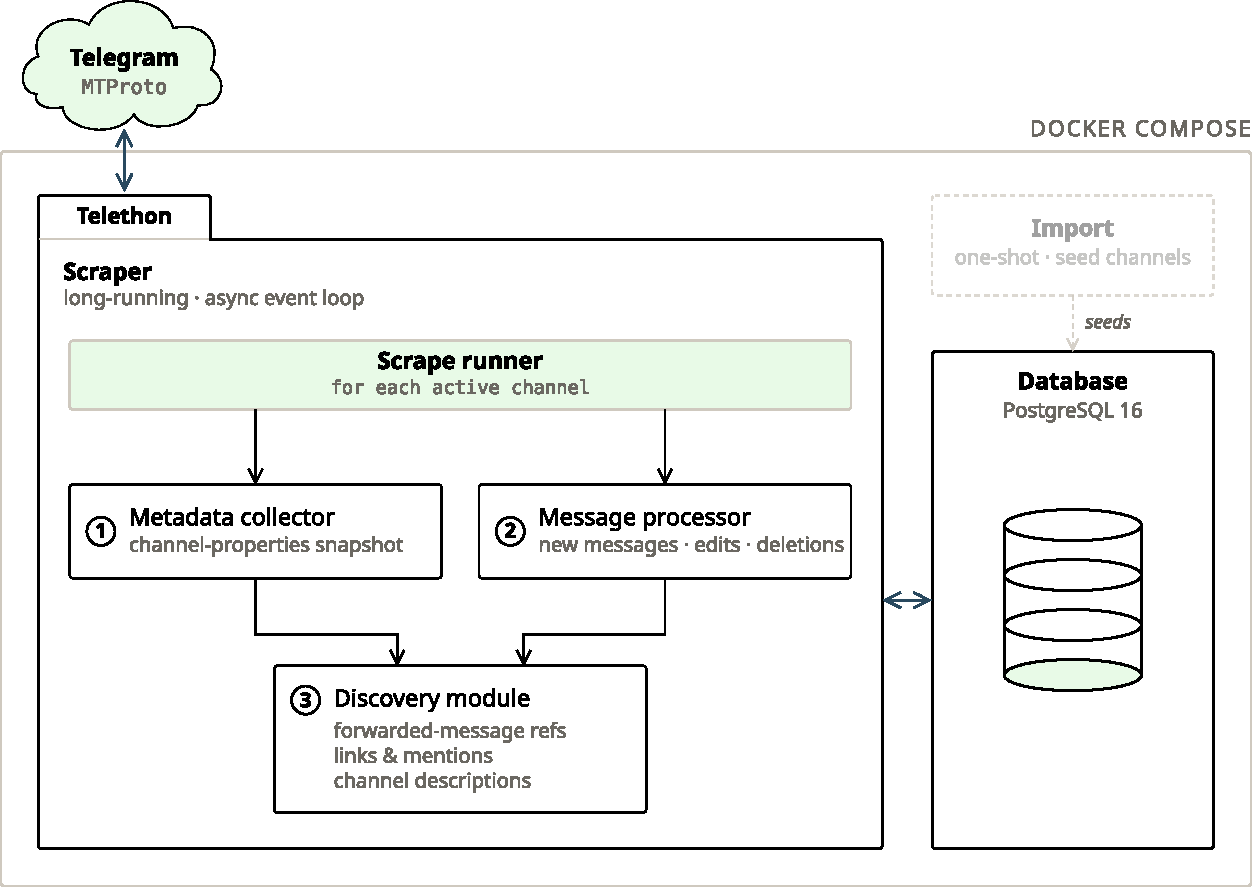
\includegraphics[width=\textwidth]{figures/architecture}
\caption[System architecture overview.]{System architecture. The scrape runner orchestrates three subsystems per channel: a metadata collector, a message processor, and a discovery module. Telethon mediates all communication with Telegram's MTProto API; PostgreSQL stores the collected data. The application is packaged as three Docker Compose services: the database, a one-time import job, and the scraper.}
\label{fig:architecture}
\end{figure}

%----------------------------------------------------------------------
\section{System Architecture}
\label{sec:architecture}
%----------------------------------------------------------------------

The system is implemented in Python using the Telethon library~\cite{telethon2026} for communication with Telegram's MTProto API.
Data is stored in a PostgreSQL~16 database, and the entire application is deployed via Docker Compose with three services: the database, a one-time channel-import job, and the scraper itself.

The scraper is structured as an asynchronous application built on Python's \texttt{asyncio} event loop.
At the top level, a \emph{scrape runner} orchestrates a continuous loop of crawl runs.
Each run iterates over the current set of active channels, and for each channel the runner invokes three subsystems in sequence: (1)~a \emph{metadata collector} that takes a snapshot of the channel's current properties, (2)~a \emph{message processor} that fetches new messages, detects edits, and identifies deletions, and (3)~a \emph{discovery module} that extracts references to previously unseen channels from forwarded messages, in-text links, and channel descriptions.

Communication with the Telegram API is subject to strict rate limits.
The scraper handles \texttt{FloodWaitError} responses by sleeping for the server-requested duration, and configurable jittered delays are inserted between API calls and between channels to reduce the likelihood of triggering rate-limit penalties.

%----------------------------------------------------------------------
\section{Telegram API and Client Library}
\label{sec:tools}
%----------------------------------------------------------------------

Telegram exposes two officially supported interfaces, and the choice between them constrains every subsequent design decision.

The \emph{Bot API}\footnote{\url{https://core.telegram.org/bots/api}} is a high-level HTTP-based interface designed for chatbot development.
It permits reading messages from groups or channels where the bot has been explicitly added, but it does not support historical message retrieval or channel discovery, ruling it out for large-scale public-channel crawling.

The \emph{MTProto API}\footnote{\url{https://core.telegram.org/api}} is Telegram's native binary protocol.
It exposes the full range of client functionality (channel search, message iteration with offset-based pagination, metadata retrieval, and entity resolution), making it the interface of choice for research-oriented scraping.
However, the MTProto API requires an authenticated \emph{user} session and is subject to strict rate limits; excessive request volumes can trigger temporary or permanent account restrictions.
We adopt MTProto despite the account-ban risk because the only alternative (the Bot API) cannot iterate the message history of a channel the bot has not been added to, and channel operators in the wild do not add third-party bots. MTProto is therefore not a preference but the only research-viable interface, and every prior dataset reviewed in Section~\ref{sec:telegram-datasets} reached the same conclusion. The risk is mitigated operationally by a dedicated secondary account and the rate-limit handling described in Section~\ref{sec:robustness}.

Two Python client libraries exist for the MTProto protocol: \textbf{Telethon}~\cite{telethon2026} and \textbf{Pyrogram}~\cite{pyrogram2024}.
Table~\ref{tab:tool-comparison} compares these alongside two other tools that are sometimes mentioned in the context of Telegram data collection but are not suitable for large-scale channel scraping.

\textbf{Telethon} is the most widely used Python MTProto library.
It provides an asynchronous abstraction over the raw protocol, supporting operations such as \texttt{iter\_messages}, \texttt{get\_messages}, and \texttt{get\_entity} that form the backbone of most Telegram scrapers in the literature~\cite{baumgartner2020,lamorgia2025,blas2025,propaganda2025}.
Telethon's \emph{takeout session} feature wraps requests in a mode that Telegram treats with relaxed flood limits, which is critical when iterating through hundreds of thousands of channels.
The library also caches entity access hashes in a local SQLite session file, eliminating redundant username-resolution calls on subsequent crawl runs.

\textbf{Pyrogram} offers a similar feature set with a more object-oriented API, but its maintenance status is the decisive concern: at the time of writing, no new release has appeared on PyPI in over 12~months and the GitHub repository shows no recent activity~\cite{pyrogram2024}.
For a long-running scraping project, an unmaintained MTProto library is a serious risk, as Telegram periodically updates its API layer and a library that does not track these changes will eventually fail to connect.
Pyrogram also lacks takeout session support, meaning the scraper cannot request relaxed flood limits for bulk export.

Two other tools warrant brief mention.
\textbf{telegram-export}~\cite{telegramexport2020} is an archived, unmaintained command-line tool (built on Telethon) designed for personal chat backup rather than channel discovery.
\textbf{python-telegram-bot}~\cite{pythontelegrambot2026} wraps the HTTP Bot~API, which cannot browse public channels or iterate their message histories, making it unsuitable for this use case.

\begin{table}[htbp]
\centering
\caption{Comparison of Python tools for Telegram data collection.}
\label{tab:tool-comparison}
\small
\begin{tabular}{@{}lcccc@{}}
\toprule
 & \textbf{Telethon} & \textbf{Pyrogram} & \textbf{telegram-export} & \textbf{PTB} \\
\midrule
Protocol        & MTProto & MTProto & MTProto & Bot API \\
Maintained      & Yes     & No      & No (archived) & Yes \\
Takeout support & Yes     & No      & No      & N/A \\
Licence         & MIT     & LGPL-3.0 & MPL-2.0 & LGPL-3.0 \\
Academic use    & Extensive & Occasional & None & None \\
\bottomrule
\end{tabular}
\end{table}

Our scraper is built on Telethon and inherits its rate-limit handling, including automatic sleep on \texttt{FloodWaitError} responses. All observations of API behaviour reported in this chapter (for example, the scoping semantics of \texttt{result.total} discussed in Section~\ref{sec:combined-pass}) were made against Telethon as pinned in the project's \texttt{pyproject.toml} at the time of data collection.

%----------------------------------------------------------------------
\section{Storage Back-End}
\label{sec:storage}
%----------------------------------------------------------------------

The storage back-end has to support the two workloads this system was designed for: bursty bulk inserts during crawl runs (hundreds of thousands of channels, hundreds of millions of messages, with append-only metadata and edit-history snapshots) and analytical queries for downstream study (temporal aggregations, forwarding-graph traversals, cross-channel joins). We do not claim these are the workloads of all Telegram scrapers; they are the workloads of \emph{this} scraper, and the back-end choice is justified against them. The two workloads do not necessarily run simultaneously: offline analyses can be performed on a static snapshot after a crawl run completes. However, a back-end that supports both concurrently on a single machine simplifies deployment and enables online monitoring or incremental analyses alongside the scraper without the overhead of exporting to a secondary system. We surveyed four candidate systems before settling on PostgreSQL; the comparison is summarized in Table~\ref{tab:db-comparison}.

\textbf{PostgreSQL}~\cite{postgresql2026} is a mature relational database with strong ACID guarantees, native JSONB support, and a rich indexing ecosystem (B-tree, GIN, GiST). Its \texttt{COPY} interface sustains the scraper's bulk-insert throughput, while its query planner, window functions, and recursive CTEs make temporal aggregations and forwarding-chain traversals expressible in standard SQL. The extension ecosystem (e.g., \texttt{pg\_trgm} for fuzzy text, pgvector for embedding-based similarity) provides a growth path without migrating to a different system.

\textbf{MongoDB}~\cite{mongodb2026} is the document store used in the original TGDataset paper~\cite{lamorgia2025}. Its schema-less model maps naturally onto the dict-like objects returned by Telethon, and GridFS offers a built-in mechanism for storing large binary files. However, the analytical workload is its weak point: aggregation pipelines are harder to write and optimize than equivalent SQL, and \texttt{\$lookup}-based cross-collection joins do not benefit from the same planner optimizations as relational joins. More critically, a nested schema that embeds all messages of a channel inside a single document would quickly exceed the 16\,MB BSON document size limit; promoting messages to their own collection recreates a relational structure but without referential integrity or standard SQL.

\textbf{SQLite}~\cite{sqlite2026} offers zero-configuration, single-file storage and is attractive for its portability, but it permits only one writer at a time. This would cause scraping and concurrent analytical queries to block one another, and its performance at the 500\,M-message scale degrades without manual partitioning across multiple database files. SQLite remains useful as a format for distributing read-only dataset snapshots, but not as the primary store.

\textbf{DuckDB}~\cite{duckdb2019} is an in-process columnar analytical engine with vectorized execution, making it extremely fast for full-table scans and aggregations. It is, however, designed for bulk-load-then-query patterns rather than for the steady stream of inserts characteristic of a long-running scraper: it has no concurrent-write support and costly \texttt{UPDATE}/\texttt{DELETE} operations. It is well suited as an optional analytical companion (its \texttt{postgres\_scanner} extension can query a live PostgreSQL instance), but not as the ingestion path.

We therefore adopt PostgreSQL~16 as the primary store. PostgreSQL is acknowledged to be slower than DuckDB for pure analytical scans and heavier to operate than SQLite; we accept both trade-offs because our workload mixes steady ingestion with concurrent reads, which is the pattern PostgreSQL's MVCC concurrency model is designed for. The relational model captures channels, metadata snapshots, messages, and edit histories as separate-but-related entities linked by foreign keys, and the remaining bottleneck (analytical speed) is addressable by attaching DuckDB via \texttt{postgres\_scanner} for ad-hoc analysis without changing the ingestion path. The schema that realizes these choices is detailed in Section~\ref{sec:schema}.

\begin{table}[htbp]
\centering
\caption{Comparison of candidate storage back-ends.}
\label{tab:db-comparison}
\small
\begin{tabular}{@{}lccc@{}}
\toprule
 & \textbf{PostgreSQL} & \textbf{MongoDB} & \textbf{SQLite} \\
\midrule
Bulk write throughput   & Excellent (\texttt{COPY}) & Good            & Fair           \\
Concurrent read/write   & Full MVCC                 & Full MVCC       & Single writer  \\
Analytical query speed  & Good                      & Mediocre        & Fair           \\
SQL support             & Full                      & None (MQL)      & Full           \\
Graph/recursive queries & Recursive CTEs            & \texttt{\$graphLookup} & Recursive CTEs \\
500\,M+ row viability   & Proven                    & Proven          & Strained       \\
Operational complexity  & Moderate                  & Moderate        & Zero           \\
\bottomrule
\end{tabular}
\end{table}

%----------------------------------------------------------------------
\section{Channel Discovery}
\label{sec:channel-discovery}
%----------------------------------------------------------------------

Channel discovery is built on snowball sampling, a chain-referral technique in which an initial set of seed entities expands iteratively by following social connections to discover previously unknown entities~\cite{goodman1961}.
Telegram's forwarding mechanism makes this technique particularly well suited to channel discovery: there is no centralized directory of public channels, but forwarded messages carry explicit references to their source channels, providing a built-in traversal link.
The known biases and limitations of snowball sampling as applied here are discussed in Section~\ref{sec:limitations}.

Starting from a user-provided set of seed channels, the scraper discovers new channels through three sources:

\begin{enumerate}
    \item \textbf{Forwarded messages.} When a message is forwarded from another channel, Telegram's API includes the source channel's numeric identifier in the \texttt{fwd\_from} field.
    These identifiers can be inserted into the database directly without additional API calls.

    \item \textbf{Links and mentions in message text.} The scraper applies regular expressions to extract \texttt{t.me/} URLs and \texttt{@username} mentions from the body of each message.
    A set of known false-positive paths (e.g., \texttt{joinchat}, \texttt{addstickers}, \texttt{share}) is filtered out.

    \item \textbf{Channel descriptions.} The same link-extraction logic is applied to each channel's ``about'' text, which is retrieved as part of the metadata snapshot.
\end{enumerate}

\begin{figure}[htbp]
\centering
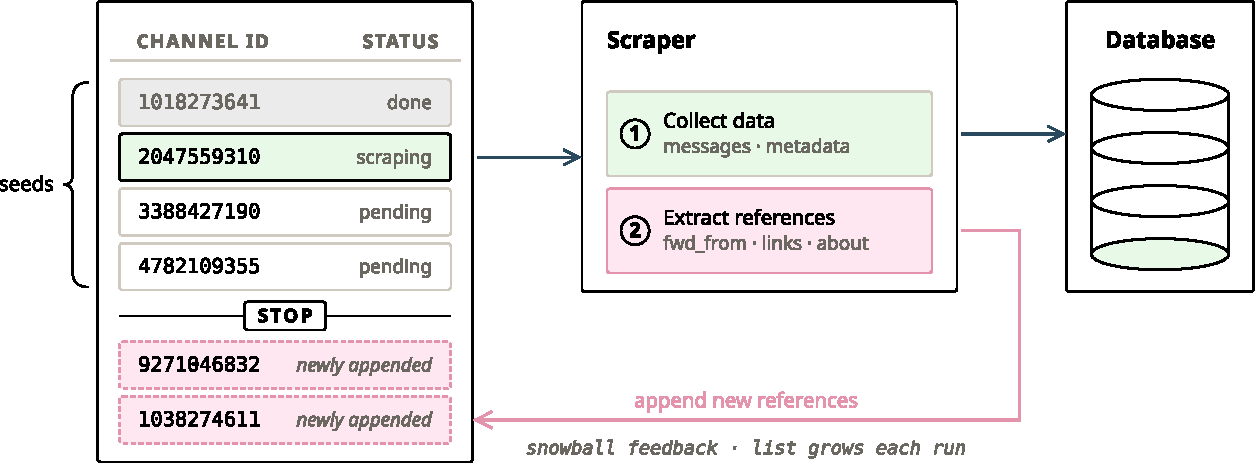
\includegraphics[width=\textwidth]{figures/snowball}
\caption[Snowball discovery loop.]{Snowball discovery loop. The scraper reads the next pending channel from the database-backed list, records its messages and metadata, extracts references to previously unseen channels from forwards, in-text links, and channel descriptions, and appends them to the list. Newly appended entries (below the run's STOP marker) are scraped on the following run.}
\label{fig:snowball}
\end{figure}

Forward-discovered channel IDs are registered in the database immediately, since Telethon provides the numeric identifier at no extra cost.
Username-based discoveries, by contrast, require a \texttt{contacts.ResolveUsername} API call to map the username to a channel ID.
The scraper implements a batched resolution mechanism: discovered usernames are queued in an \texttt{unresolved\_references} table (Section~\ref{sec:schema}) and resolved with doubled inter-request delays, while permanently invalid usernames (e.g., deleted or private channels) are marked and excluded from future attempts.

In practice, however, username resolution is disabled in our deployment because Telegram imposes strict rate limits on \texttt{contacts.ResolveUsername}.
The daily limit is documented at roughly 200 calls~\cite{tginfolimits}, and exceeding it triggers a \texttt{FLOOD\_WAIT\_X} error~\cite{telegramapierrors} with mandatory wait times that can reach 24 hours.
For a continuously running scraper that already consumes its rate budget on message retrieval, spending part of that budget on username resolution is impractical.
Channel discovery therefore relies exclusively on forwarded-message identifiers, which the API provides at no additional cost.
Disabling username resolution introduces a known sampling bias: channels that are only reachable through \texttt{@}-mentions or \texttt{t.me/} links, without ever being forwarded, are under-sampled. We accept this bias because the alternative (spending the rate-limit budget on resolution calls) would halt message collection outright, and because forwarded-message references are empirically the dominant discovery channel on our deployment, as reported in Chapter~\ref{chap:results}. The bias is revisited in the Limitations section of Chapter~\ref{chap:results}.

Because channels discovered during a run are added to the database but not to the current run's channel list, the snowball expansion takes effect on the \emph{next} run.
This design avoids unbounded growth of a single run and ensures that the channel list for each run is fixed at the start, simplifying crash recovery (Section~\ref{sec:robustness}).

Figure~\ref{fig:snowball} summarizes the resulting feedback loop: each run iterates over a channel list drawn from the database; for every channel the scraper collects messages and metadata, extracts references to previously unseen channels, and appends them to the list for use by the next run.

%----------------------------------------------------------------------
\section{Database Schema}
\label{sec:schema}
%----------------------------------------------------------------------

The database schema is designed around four requirements: preserving Telegram's native identifiers, supporting longitudinal metadata tracking, recording message edit histories, and enabling crash-safe incremental collection.
Eight tables, whose relationships are summarized in Table~\ref{fig:erd}, serve three functional groups: channel identity and metadata, message storage and edit history, and operational bookkeeping.

\begin{figure}[htbp]
\centering
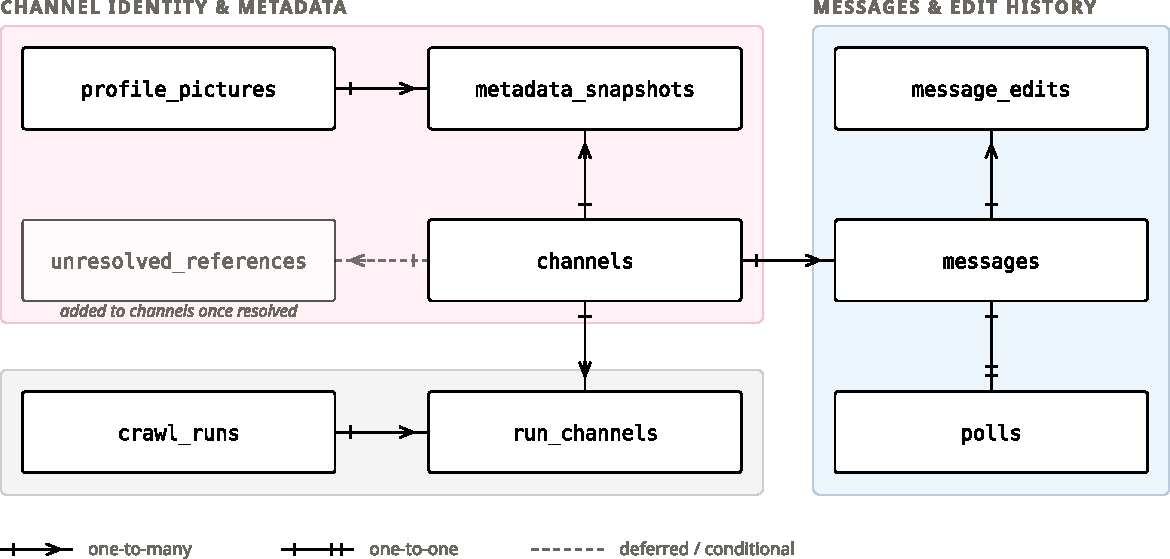
\includegraphics[width=\textwidth]{figures/erd}
\caption[Database schema entity-relationship diagram.]{Entity-relationship diagram of the database schema. Solid arrows denote one-to-many or one-to-one relationships (see legend); \texttt{unresolved\_references} (dashed border) is linked to \texttt{channels} conditionally, once a username has been resolved to a channel ID. Three functional groups are shaded: channel identity and metadata (top left), messages and edit history (right), and operational bookkeeping (bottom).}
\label{fig:erd}
\end{figure}

\subsection{Channel identity and metadata}

\paragraph{Channels.}
The \texttt{channels} table stores one immutable identity record per channel, keyed by Telegram's native signed 64-bit channel ID.
Each row records when the channel was created, when the scraper first encountered it, and how it was discovered (\texttt{seed}, \texttt{forward}, \texttt{mention}, \texttt{manual}, or \texttt{linked\_group}).
Three boolean flags support the scraping cycle: \texttt{is\_active} acts as a circuit breaker that disables a channel after a configurable number of consecutive failures, \texttt{initial\_pull\_complete} tracks whether the first full historical download has finished, and \texttt{needs\_recheck} is set before processing and cleared on success, surviving crashes to trigger a forced recheck on restart.
A \texttt{linked\_to\_channel\_id} foreign key records the parent for channels that serve as discussion groups.

\paragraph{Metadata snapshots.}
The \texttt{metadata\_snapshots} table stores one row for each channel on every crawl visit, forming the core of the longitudinal tracking.
Each snapshot captures the channel's public identity (username, title, description), its subscriber count, trust-related flags set by Telegram (scam, verified, restricted, fake), a reference to the active profile picture, and the linked discussion-group ID.
A dedicated \texttt{is\_private} flag marks snapshots recorded when the channel returned a \texttt{ChannelPrivateError}; in these rows all other fields are null.
By diffing consecutive snapshots one can detect name changes, description edits, subscriber growth or decline, profile-picture swaps, and transitions to or from private status.

\paragraph{Profile pictures.}
Channel profile pictures are stored in a content-addressable \texttt{profile\_pictures} table, keyed by the SHA-256 hash of the raw image bytes.
Each row also stores a 64-bit DCT-based perceptual hash and a 64-bit difference hash, enabling near-duplicate detection across channels.
Idempotent insertion (\texttt{ON CONFLICT DO NOTHING}) ensures that the same image is stored only once, even when multiple snapshots reference it.
Photo-change detection is optimized by comparing the \texttt{photo\_id} (a lightweight integer exposed by the API) between consecutive snapshots; the image bytes are downloaded only when a change is detected.

\subsection{Messages and edit history}

\paragraph{Messages.}
The \texttt{messages} table is the central fact table, keyed by the composite primary key \texttt{(channel\_id, message\_id)}.
Table~\ref{tab:messages} summarizes the information stored for each message, grouped thematically.
Columns are physically ordered by descending alignment size (8-byte, 4-byte, 1-byte, variable-length) to minimize PostgreSQL's inter-column padding overhead, which would otherwise waste approximately 7--8~bytes per row.
The variable-length columns (\texttt{text} for message bodies, \texttt{jsonb} for entities and reactions) keep PostgreSQL's default \texttt{EXTENDED} storage strategy. \texttt{EXTENDED} declares a column \emph{eligible} for compression and for out-of-line storage in the TOAST side-table; neither is applied until the row would otherwise exceed the tuple threshold (\texttt{TOAST\_TUPLE\_THRESHOLD}, roughly 2\,kB). Short messages therefore remain inline and uncompressed, while long ones are compressed first and moved out-of-line only if still too large. This behaviour matches our workload: most Telegram posts are short and cost nothing to read, while the rare long post does not bloat the main heap.

\begin{table}[htbp]
\centering
\caption{Information stored per message in the \texttt{messages} table, grouped by theme.}
\label{tab:messages}
\small
\begin{tabular}{@{}lp{8.5cm}@{}}
\toprule
\textbf{Group} & \textbf{What is stored} \\
\midrule
Timestamps      & Publication date, last edit date, and the time the message was first collected by the scraper. \\
Content         & Raw message text (PostgreSQL \texttt{text}), structured entities (URLs, mentions, formatting as JSONB), a media-type indicator, a service-action type for system messages such as channel creation or pin events, and a JSONB payload that preserves the action's constructor arguments for actions that carry one. Media files themselves are not downloaded: see the rationale below. \\
Authorship      & Poster's numeric user or channel ID and an optional author-signature string. \\
Engagement      & View count, forward count, reply count, pinned status, and per-emoji reaction counts (JSONB). \\
Forwarding      & Whether the message is a forward, the source channel ID and message ID, the original posting date, and a display name for hidden or deleted sources. \\
Threading       & Reply-to message ID, top-level thread ID, a comment-thread flag, and an album-grouping ID for multi-media posts. \\
Deletion        & A deleted flag and a timestamp recording when the deletion was detected (Section~\ref{sec:combined-pass}). Deleted rows are retained to preserve the historical record. \\
\bottomrule
\end{tabular}
\end{table}

Media files attached to messages (photos, videos, documents) are deliberately not downloaded. Storing media at dataset scale would additional storage, raises legal sensitivity around potentially copyrighted or illicit content, and is out of scope for a study whose primary unit of analysis is channel metadata and text. The stored media-type indicator is sufficient to reconstruct any media file on demand via the Telegram API, should a downstream study require it.

\paragraph{Message edits.}
The \texttt{message\_edits} table preserves previous versions of edited messages.
When an edit is detected, the current content of the \texttt{messages} row (text, entities, media flag, and media type) is copied here before the row is overwritten with the new version.
The \texttt{messages} table therefore always holds the latest version, while the full edit history is available by joining with \texttt{message\_edits} and ordering by the \texttt{captured\_at} timestamp.

\paragraph{Polls.}
Messages whose \texttt{media\_type} is \texttt{poll} are accompanied by a row in the \texttt{polls} table, keyed by the same \texttt{(channel\_id, message\_id)} composite key.
Each row stores the stable Telegram poll identifier, the question text and its formatting entities, and a JSONB \texttt{answers} array whose elements record option text, raw option bytes (base64-encoded), vote tallies, and, for quizzes, a flag indicating the correct answer.
Four boolean flags characterize the poll configuration: \texttt{is\_closed}, \texttt{is\_quiz}, \texttt{is\_multiple} (whether multiple answers may be selected), and \texttt{is\_public\_voters} (whether individual votes are visible to subscribers).
Optional fields capture the close schedule (\texttt{close\_period}, \texttt{close\_date}), the aggregate voter count, and the quiz explanation text (\texttt{solution}).
The table is latest-only: re-observation overwrites the mutable fields (tallies, \texttt{is\_closed}) in place and advances \texttt{captured\_at}, so the row always reflects the most recent snapshot rather than a full history of vote counts.

\subsection{Operational bookkeeping}

\paragraph{Crawl runs and run channels.}
The \texttt{crawl\_runs} table records every scraping or alignment run with its type, status, start and end timestamps, progress counters (channels attempted, channels completed, messages collected), and, for alignment runs, the cutoff timestamp.
A JSONB \texttt{config\_snapshot} column preserves the scraper's configuration at the time of each run for reproducibility.
The associated \texttt{run\_channels} table persists the ordered list of channels for each run, with a per-channel status (\texttt{pending}, \texttt{completed}, \texttt{partial}, or \texttt{error}). The \texttt{partial} status records that the channel was processed but its pull was interrupted by a sustained network outage; see Section~\ref{sec:robustness}.
Together, these two tables enable crash recovery: on restart the scraper queries for the most recent incomplete run, retrieves its pending channels, and resumes from where it left off.

\paragraph{Unresolved references.}
The \texttt{unresolved\_references} table queues usernames discovered via links and mentions that have not yet been resolved to channel IDs.
Each entry tracks the number of resolution attempts and the timestamp of the last attempt, implementing a retry-with-backoff strategy.
As noted in Section~\ref{sec:channel-discovery}, the resolution mechanism is not used in our deployment due to Telegram's rate limits on \texttt{contacts.ResolveUsername}; the table nonetheless records the discovered usernames for potential offline or manual resolution.

%----------------------------------------------------------------------
\section{Scraping Cycle}
\label{sec:scraping-cycle}
%----------------------------------------------------------------------

The scraper operates in a continuous loop of crawl runs, with the database as the single source of truth for which channels to process.

\paragraph{Run initialization.}
At the start of each run, the scraper queries the \texttt{channels} table for all rows where \texttt{is\_active = true}, creates a new entry in \texttt{crawl\_runs}, and persists the ordered channel list to \texttt{run\_channels}.
The list is built from two concatenated segments. The first segment contains all channels that have already been scraped in a previous run, kept in a fixed order that simply grows as new channels graduate into it. The second segment contains all channels not yet scraped (the seed set on the very first run, plus any references discovered since), and is shuffled at random before the start of the run.
Shuffling the unscraped segment matters because a single channel can contribute hundreds of new references in one visit (through forwards, in-text links, and its description); without randomization those references would be processed back-to-back, skewing the sample toward large or densely-connected forwarding graphs. Interleaving them with references discovered by other channels diffuses this locality.
Figure~\ref{fig:snowball-list} shows how this two-part structure evolves across successive runs: the ``seen'' prefix accumulates monotonically while each fresh batch of discovered references is shuffled before being appended.
The channel list is fixed for the duration of the run; channels discovered during processing are added to the database but only appear in subsequent runs.

\begin{figure}[htbp]
\centering
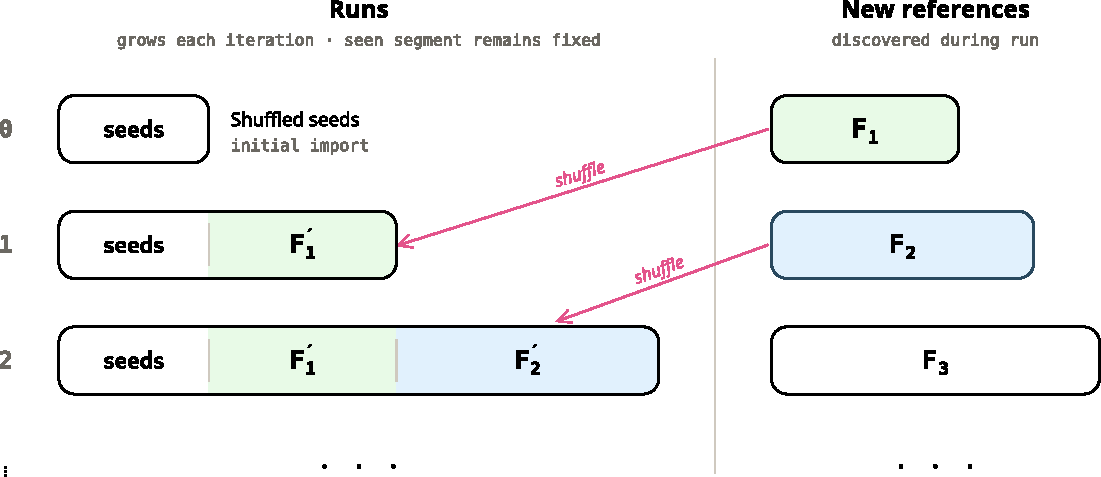
\includegraphics[width=\textwidth]{figures/snowball_list}
\caption[Scraping-list growth across runs.]{Evolution of the scraping list across successive runs. In run~0 the list contains only seeds, shuffled. After run~0, the seeds move into the fixed ``seen'' prefix and the new references $F_1$ discovered during the run are shuffled into the unscraped segment as $F'_1$ for run~1. This pattern repeats: the seen prefix grows monotonically while each fresh batch of discovered references is shuffled before being appended.}
\label{fig:snowball-list}
\end{figure}

\paragraph{Per-channel processing.}
For each channel, the scraper performs three steps:
\begin{enumerate}
    \item \textbf{Metadata snapshot.} A single \texttt{GetFullChannelRequest} API call retrieves the channel entity and its extended metadata, which is inserted as a new row in \texttt{metadata\_snapshots}.
    If the profile picture has changed (detected via \texttt{photo\_id} comparison), the new image is downloaded, hashed, and stored.

    \item \textbf{Message processing.} The combined pass described in Section~\ref{sec:combined-pass} fetches new messages, detects edits on previously stored messages, and identifies deletions.

    \item \textbf{Channel discovery.} Forward references and link-based usernames extracted during message processing, together with links from the channel description, are registered or queued for resolution.

    \item \textbf{Linked discussion group (conditional).} A broadcast channel can have an associated discussion group attached to it; messages posted by subscribers in that group, threaded under a broadcast post, are what Telegram exposes as ``comments'' on the post. If the parent's metadata snapshot reports such a linked group and comment collection is enabled, the group is recorded in \texttt{channels} with source \texttt{linked\_group} and a back-pointer to the parent. The same three steps above are then applied to the linked group as part of the same per-channel iteration, sharing the parent's run identifier and (during alignment) cutoff timestamp. The back-pointer marks the linked group as a child of an already-queued channel, so it is excluded from the regular scrape queue and is visited only as part of its parent's turn, which preserves the channel/group pair as a single unit of work.
\end{enumerate}

After each channel completes, its \texttt{run\_channels} row is updated from \texttt{pending} to \texttt{completed} (or \texttt{partial} or \texttt{error}), and the run-level counters are incremented.
If a shutdown signal is received mid-iteration, the run is marked as \texttt{interrupted} and the remaining channels are left as \texttt{pending} for resumption.

\paragraph{Inter-run behavior.}
Runs repeat indefinitely.
Each new run sees the full, up-to-date channel list, including any channels discovered during previous runs.
Before starting a fresh run, the scraper checks for incomplete runs from prior sessions and resumes them first (Section~\ref{sec:robustness}).

%----------------------------------------------------------------------
\section{Combined Pass: New Messages, Edit Detection, and Deletion Detection}
\label{sec:combined-pass}
%----------------------------------------------------------------------

The three core message-level operations (fetching new content, detecting edits, and identifying deletions) are performed together in a single combined pass per channel, minimizing redundant API calls.
The pass branches based on whether deletions are detected.

\subsection{Setup}
\label{sec:combined-setup}

For each channel, two values are derived from the \texttt{messages} table at query time:
\begin{itemize}
    \item \texttt{highest\_id}: the maximum \texttt{message\_id} stored for this channel.
    \item \texttt{message\_count}: the number of non-deleted messages whose \texttt{message\_id} lies in the range $[0, \texttt{highest\_id}]$.
\end{itemize}

\begin{figure}[htbp]
\centering
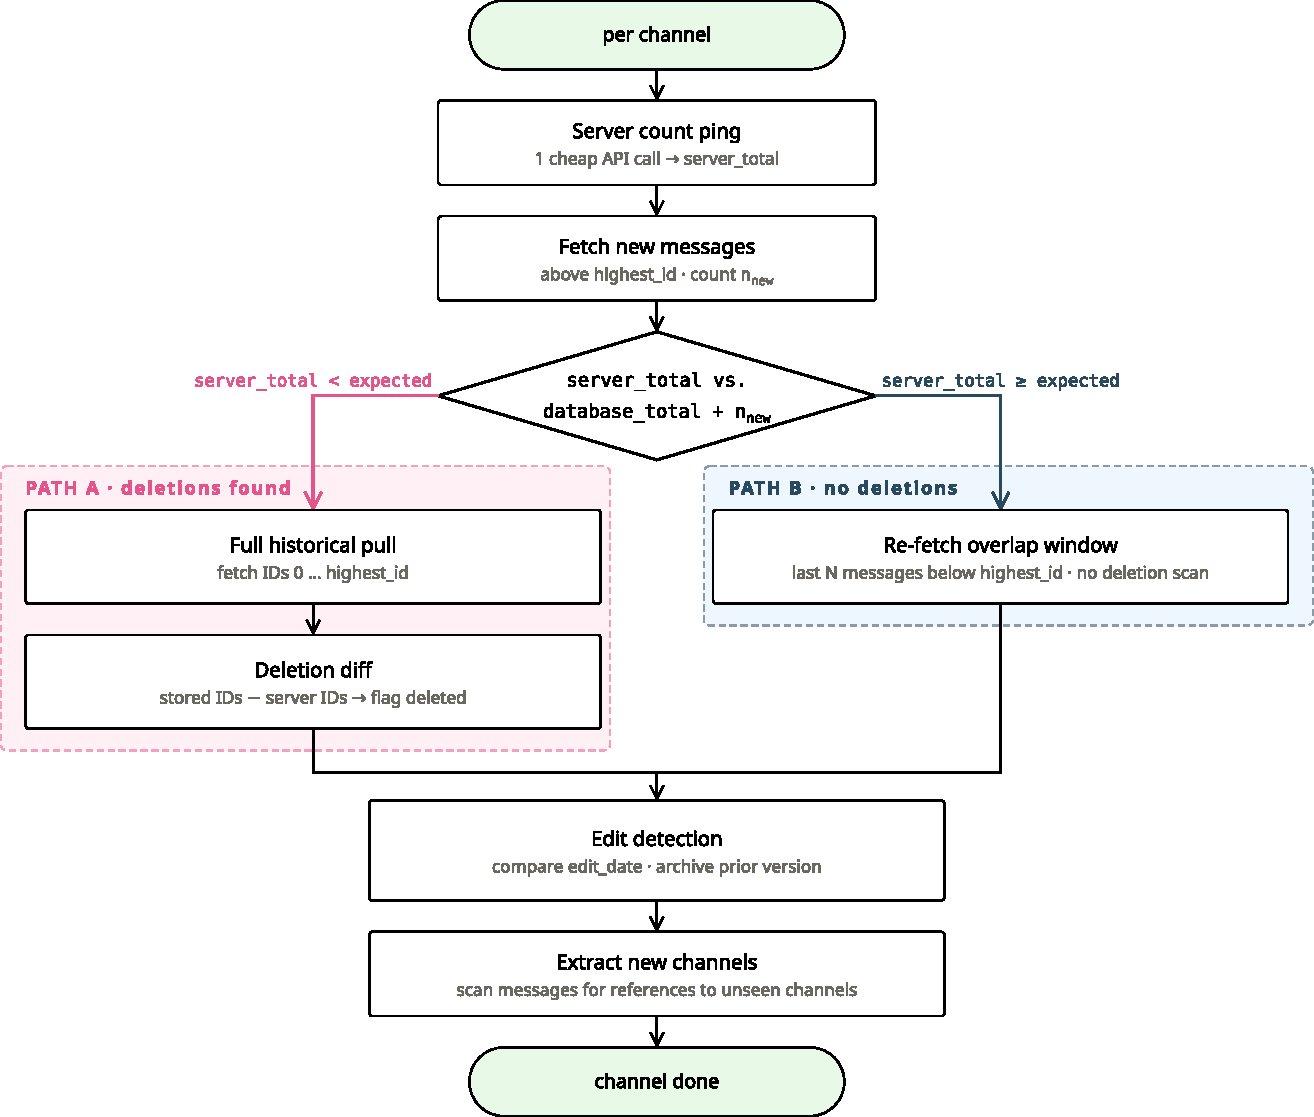
\includegraphics[width=\textwidth]{figures/combined-pass}
\caption[Combined-pass flowchart.]{Combined pass for a single channel. A cheap preliminary ping yields \texttt{server\_total}; after the new-message fetch, the comparison against $n_{\text{expected}}$ branches into Path~A (full historical pull with deletion diff) or Path~B (re-fetch of the overlap window). Edit detection is a shared subroutine: both paths feed every fetched message into the same \texttt{edit\_date} comparison.}
\label{fig:combined-pass}
\end{figure}

If \texttt{highest\_id} is null (no messages have ever been collected), the scraper performs a full initial pull, paginating through all messages from newest to oldest and committing each batch to the database as it arrives.

\subsection{Deletion count check}

A single cheap API call retrieves the server-reported total message count:
\begin{lstlisting}[language=Python]
result = await client.get_messages(entity, limit=0)
server_total = result.total
\end{lstlisting}

We observed empirically that \texttt{result.total} always returns the \emph{full} channel message count regardless of any \texttt{min\_id} or \texttt{max\_id} parameters: passing \texttt{max\_id=100}, \texttt{max\_id=10000}, or no bound at all yields the same scalar.
The count cannot therefore be scoped to a historical range, and new messages must be fetched and counted before the comparison can be made.
The flip side of this constraint is what makes the strategy work: because \texttt{server\_total} is channel-global, a single equality between \texttt{server\_total} and the locally derived expected count rules out deletions \emph{anywhere} in the channel, not just above some cutoff. This is the guarantee that justifies the cheap path~B described next.

\subsection{Branching logic}

After fetching new messages (those with IDs above \texttt{highest\_id}) and counting them as $n_{\mathrm{new}}$, the expected count is computed as $n_{\mathrm{expected}} = \texttt{message\_count} + n_{\mathrm{new}}$.
The pass then branches:

\paragraph{Path A: deletions detected ($\texttt{server\_total} < n_{\mathrm{expected}}$).}
At least one message has been removed somewhere in $[0, \texttt{highest\_id}]$, and the count check by itself cannot say where. The number of missing messages, however, is known exactly: because \texttt{server\_total} is channel-global, the deficit $\Delta = n_{\mathrm{expected}} - \texttt{server\_total}$ is precisely how many stored IDs the server no longer returns. Locating them in full requires a historical pull that re-fetches every message from ID~0 to \texttt{highest\_id}. On a large channel this sweep is costly, and running it on every visit that detects even a single deletion would dominate the per-channel API cost.

Under the assumption that most deletions are recent, Path~A first attempts a cheap recent-window scan before committing to the full sweep. It re-fetches only the same overlap window of $N$ messages below \texttt{highest\_id} that Path~B uses for edits, and diffs the stored IDs within that window against the IDs the server returns for it. If the number of in-window deletions is at least $\Delta$, then every missing message lies inside the window: the entire deficit is accounted for, none can lie below it, and the full pull is skipped. Only when fewer than $\Delta$ deletions are found in the window, leaving part of the deficit unexplained, does the scraper fall back to the full historical pull from ID~0.

The threshold is ``at least $\Delta$'' rather than ``exactly $\Delta$'' by design. A deletion occurring inside the window between the count ping and the window scan can push the in-window count above $\Delta$; those extra IDs are genuinely absent from the window, which was scanned in full, so marking them and skipping remains correct. The test is unsafe only in the opposite direction, when $\Delta$ understates the true number of deletions, and that can happen only if $n_{\mathrm{new}}$ was undercounted by an interrupted new-message fetch. The fast path is therefore attempted only when that fetch completed cleanly and the channel's stored history is already known to be contiguous ($\texttt{initial\_pull\_complete} = \text{true}$); a forced crash-recovery recheck (Section~\ref{sec:robustness}), where the counts cannot be trusted, bypasses the window scan and goes straight to the full historical pull.

Whichever scan runs, deletion handling is identical: IDs present in the database but absent from the scan are flagged as deleted (the rows are retained with \texttt{is\_deleted = true} and a \texttt{deleted\_at} timestamp, preserving the historical record). Edit detection is piggybacked on the fetched messages: for each that already exists in the database, the \texttt{edit\_date} is compared against the stored value, and edits are archived. On a successful fast path the overlap window is edit-scanned exactly as in Path~B.

\paragraph{Path B: no deletions ($\texttt{server\_total} \geq n_{\mathrm{expected}}$).}
Only an overlap window of $N$ messages below \texttt{highest\_id} is re-fetched (where $N$ is configurable, defaulting to~100).
These messages are checked for edits, but no deletion scan is performed: the channel-global equality already established in Section~\ref{sec:combined-pass} mathematically covers every ID in $[0, \texttt{highest\_id}]$, so re-verifying any subset of that range would be redundant. The overlap window exists purely to surface edits, which the count check cannot detect because edits do not change the message total.

The count-based heuristic has a known blind spot: if exactly as many messages are deleted as are newly posted between two visits, \texttt{server\_total} will equal $n_{\mathrm{expected}}$ and the deletion will be silently missed until a subsequent visit restores the imbalance. We accept this because the only alternative is a full-history pull on every visit. Such a pull would multiply the per-channel API cost by several orders of magnitude and make continuous crawling inefficient. Two further limitations follow from the same trade-off and are revisited in Section~\ref{sec:limitations}. First, Path~B sees no edits to messages older than the overlap window until that channel happens to enter Path~A. Second, a benign race between the count ping and the new-message pull can occasionally inflate $n_{\mathrm{expected}}$ enough to trigger a redundant (but non-corrupting) Path~A run. A related but distinct issue during alignment runs, where the cutoff timestamp applies only to the new-message fetch and not to the count ping, is discussed in Section~\ref{sec:alignment}.

\subsection{Edit detection logic}

Whenever a message is fetched (in either path), its \texttt{edit\_date} is compared against the version stored in the database:
\begin{itemize}
    \item If the stored \texttt{edit\_date} is null and the fetched one is set, or the fetched \texttt{edit\_date} is strictly newer, an edit is recorded.
    \item The current version in \texttt{messages} is copied to \texttt{message\_edits} (preserving the pre-edit content), and the \texttt{messages} row is then updated with the new content.
\end{itemize}
No additional API calls are needed: edit detection piggybacks entirely on the message fetches already required for deletion checking and new-message collection.

%----------------------------------------------------------------------
\section{Alignment Snapshots}
\label{sec:alignment}
%----------------------------------------------------------------------

A key challenge in longitudinal dataset construction is ensuring temporal consistency: when crawling thousands of channels sequentially, channels processed early in a run reflect data from a different point in time than those processed later.
Alignment snapshots address this by bringing all channels to a common cutoff timestamp.

\subsection{Trigger}

An alignment snapshot can be triggered in two ways: automatically, when a configurable interval (e.g., 30~days) has elapsed since the last alignment, or manually, by sending a \texttt{SIGUSR1} signal to the scraper process.
In both cases, the current scrape run is interrupted and marked accordingly, and a cutoff timestamp $t_c$ is set to the current time.

\subsection{Alignment processing}

A new crawl run of type \texttt{alignment\_snapshot} is created with \texttt{cutoff\_timestamp} = $t_c$.
The alignment iteration processes all channels that have been fully scraped at least once (\texttt{initial\_pull\_complete = true}).
For each channel, the same combined pass as a regular scrape is executed (Section~\ref{sec:combined-pass}), with one modification: new messages are fetched only up to $t_c$ by setting Telethon's \texttt{offset\_date} parameter.
This ensures that every channel's message history is complete up to the same point in time.
Alignment is \emph{eventually consistent}, not instantaneous: the alignment run itself takes time to traverse all channels, and during that traversal the metadata of channels processed earlier continues to drift. What the cutoff timestamp guarantees is that every channel's message stream is captured up to the same $t_c$; it does not guarantee that the metadata snapshots across channels were taken at the same wall-clock moment. This is an inherent limit of sequential single-machine scraping rather than a shortcoming of the alignment protocol, and the drift is bounded by the duration of one alignment cycle.

\paragraph{Path selection under the cutoff.}
The cutoff $t_c$ is propagated into the new-message fetch via \texttt{offset\_date}, but not into the preliminary count ping, which cannot be scoped to a historical range (Section~\ref{sec:combined-pass}). During alignment, therefore, \texttt{server\_total} reports the channel-global count at the moment the channel's turn arrives, while $n_{\mathrm{new}}$ stops at $t_c$. Any message posted in the interval $[t_c, \text{now}]$ inflates \texttt{server\_total} without inflating $n_{\mathrm{expected}}$, so the cheap check enters Path~A only when the number of genuine deletions exceeds the number of post-cutoff posts. This widens the intra-request race described in Section~\ref{sec:combined-pass} from the gap between two API calls (seconds) to the gap between the alignment trigger and the channel's turn (minutes to hours on a large channel list), and its effect is to \emph{mask} deletions rather than falsely signal them. Busy channels processed late in the alignment queue are therefore the most exposed. The asymmetry is tolerated because alignment is always followed by a fresh regular scrape (the post-alignment step described below), which runs without a cutoff and exercises an exact cheap check, so any deletion masked during alignment surfaces on the immediately following pass. Alignment also does not unconditionally force Path~A: the \texttt{needs\_recheck} flag is set on each channel as a crash-guard, but path selection reads its \emph{prior} value, so only channels whose flag was already set (for example, by an earlier crash) take Path~A regardless. Finally, the recent-window fast path within Path~A (Section~\ref{sec:combined-pass}) tests against this same understated $\Delta$, so during alignment it can skip the full pull while a deletion below the overlap window goes unmarked; like a fully masked deletion, it is recovered by the exact check on the immediately following regular scrape.

\begin{figure}[htbp]
\centering
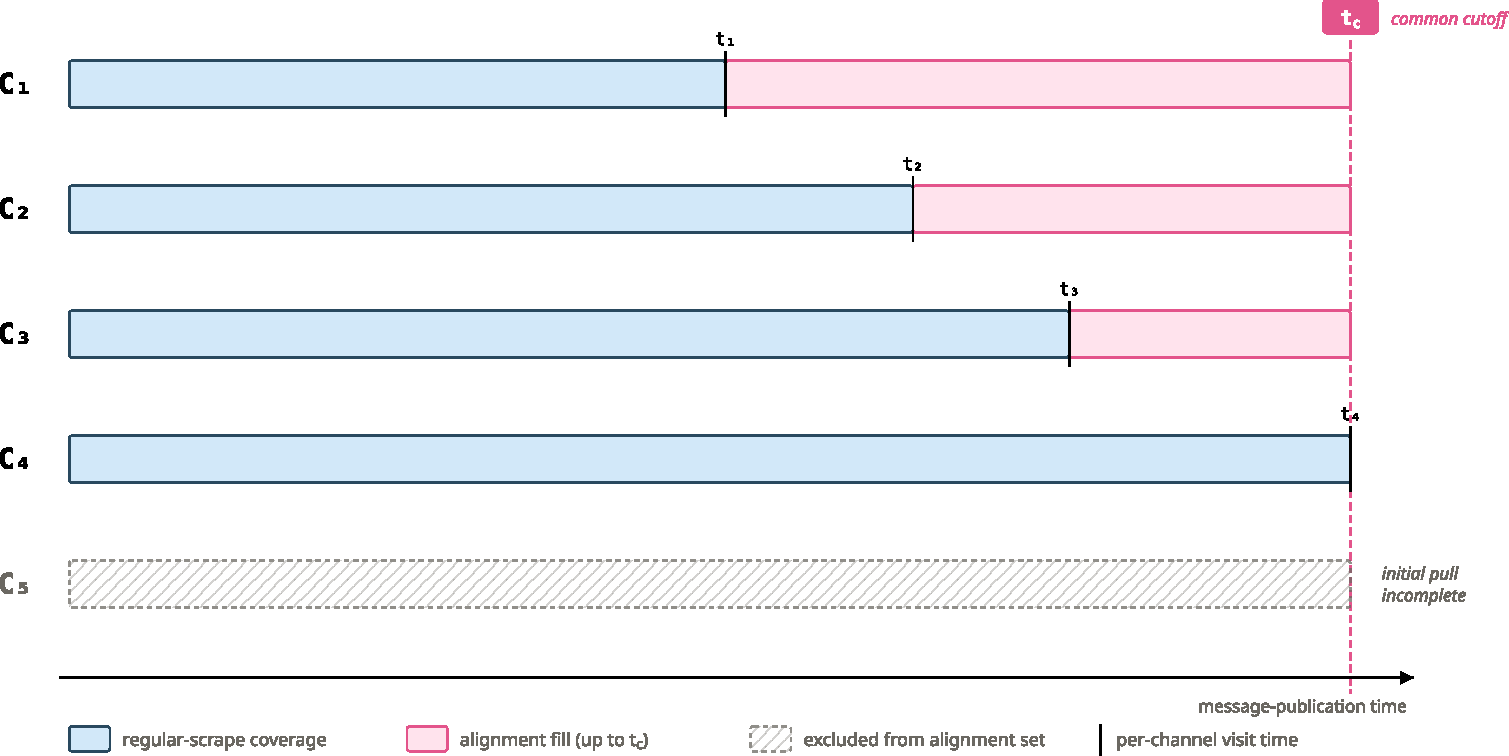
\includegraphics[width=\textwidth]{figures/alignment}
\caption[Alignment data coverage.]{What alignment guarantees, shown as per-channel message-stream coverage. The horizontal axis is message-publication time (not scraper wall-clock). During a regular scrape each channel $C_i$ is visited at a different moment $t_i$, so its data ends at a different point (blue segments). The alignment run then fills, for every channel with \texttt{initial\_pull\_complete\,=\,true}, the gap from $t_i$ up to the common cutoff $t_c$ (orange segments), so every channel's message history is complete up to the same point in time. Channels that have not completed their initial pull ($C_5$ here) are excluded from the alignment set (\texttt{get\_scraped\_channel\_ids} returns only fully scraped channels) and wait for a subsequent regular run before any future alignment can include them.}
\label{fig:alignment}
\end{figure}

\subsection{Post-alignment}

Once the alignment iteration completes, the alignment flag is cleared and a regular scrape run resumes with the full channel list, including any channels discovered during both the interrupted scrape and the alignment itself.

%----------------------------------------------------------------------
\section{Robustness}
\label{sec:robustness}
%----------------------------------------------------------------------

The scraper is designed to run continuously over weeks or months, and must tolerate network failures, process crashes, and API errors without data loss or corruption.
Several mechanisms contribute to this goal.

\paragraph{Graceful shutdown.}
The scraper installs handlers for \texttt{SIGTERM} and \texttt{SIGINT}.
When a shutdown signal is received, an asyncio event is set that is checked between batches and between channels.
The current operation is allowed to finish, the active run is marked as \texttt{interrupted}, and the process exits cleanly.

\paragraph{Crash recovery.}
Recovery operates at two levels.
At the \emph{run level}, on startup the scraper marks any leftover \texttt{running} crawl runs as \texttt{interrupted} and queries for the most recent incomplete run.
If one is found, its pending channels are retrieved from \texttt{run\_channels} and processing resumes from there.
At the \emph{channel level}, two flags on the \texttt{channels} table provide fine-grained recovery.
The \texttt{initial\_pull\_complete} flag is set to \texttt{false} until the first full historical download finishes; if a crash occurs mid-pull, the next run detects the incomplete state and fetches only the missing older messages (below the lowest stored ID) rather than re-fetching everything.
The \texttt{needs\_recheck} flag is set before a channel is processed and cleared only after all processing (including channel-discovery resolution) succeeds; if it survives a crash, the channel receives a forced full historical check on the next run.

\paragraph{Per-page persistence.}
Messages are committed to the database in batches as they arrive from the API, rather than being buffered until the end of a channel.
This minimizes data loss on crash: at most one batch of messages (configurable, default 100) can be lost. Per-message transactions would eliminate even this bounded loss, but at a cost in transaction overhead; the batch-level bound is the accepted trade-off, and any lost batch is recovered on the next run because the same messages will be re-fetched as long as they sit above the stored \texttt{highest\_id}. The scraper is designed to run as a single process on a single machine; multi-instance or distributed scraping is explicitly out of scope.

\paragraph{Per-channel error handling.}
Private and invalid channels are handled differently.
When a channel returns a \texttt{ChannelPrivateError}, the scraper records a private snapshot (Section~\ref{sec:schema}) and moves on without incrementing the error counter, since a channel that has become private may later be made public again.
For other failures (e.g., deleted or temporarily unavailable channels), the error is logged and a \texttt{consecutive\_errors} counter is incremented.
The counter resets on success; when it reaches a configurable threshold (default~2), the channel is deactivated (\texttt{is\_active = false}), preventing further wasted API calls.

\paragraph{Connection resilience.}
Before processing each channel, the scraper checks whether the Telegram client connection is still alive and reconnects if necessary.
Message iteration is protected by a per-message timeout: if no message arrives within 60~seconds, the iterator is abandoned with a partial batch rather than blocking indefinitely.
When such a timeout fires, the scraper does not advance to the next channel. Instead it parks on the current channel, force-reconnects the Telegram client, probes the API with a lightweight RPC to confirm the connection is actually live, and retries the pull in place. Retries use an exponentially growing backoff capped at a few minutes, and are repeated up to a configurable attempt cap that, at the default backoff schedule, spans roughly a full day of downtime. Each retry resumes from the partial state already on disk via the \texttt{initial\_pull\_complete} machinery (Section~\ref{sec:schema}), so progress is monotone across attempts. If the attempt cap is reached without recovery, the channel's \texttt{run\_channels} row is recorded as \texttt{partial} (rather than \texttt{completed} or \texttt{error}) and its \texttt{needs\_recheck} flag is left set, so the next run revisits it and finishes the pull.

\paragraph{Rate-limit handling.}
\texttt{FloodWaitError} responses from the Telegram API cause the scraper to sleep for the server-requested duration plus a small buffer.
During username resolution, a flood-wait sets a cooldown timestamp that suppresses further resolution attempts until the penalty period expires, preventing escalating rate-limit penalties.

%----------------------------------------------------------------------
\section{Deployment}
\label{sec:deployment}
%----------------------------------------------------------------------

The system is packaged as a Docker Compose application comprising three services.
The \textbf{database} service runs PostgreSQL~16 (Alpine), with the schema automatically applied from an initialization script on first start and data persisted in a named volume.
Version~16 is chosen over the latest major release for its maturity (several minor releases of accumulated bug fixes), its long community-support window (through November~2028), and the wider availability of compatible extensions and client libraries; none of the features introduced in subsequent major versions materially affect this workload.
The \textbf{import} service is a one-time job that populates the \texttt{channels} table with the active dataset's seed channel IDs, read from a seed file (one ID per line) whose path is supplied by an environment variable, with optional additional seeds passed inline through a second variable; it exits after completion and is not restarted. For the main corpus this seed file was the TGDataset channels~\cite{lamorgia2025}, in randomized order.
The \textbf{scraper} service runs the main application, configured via environment variables for API credentials, database connection, timing parameters (request delay, channel delay, jitter), batch size, overlap window, alignment interval, and error thresholds.
The Telethon session file, which stores the authenticated user session, is bind-mounted into the container to persist across restarts.

All configuration parameters are exposed as environment variables with documented defaults, allowing deployment-time tuning without code changes.
Table~\ref{tab:config} lists the principal parameters. The values shown in the \textit{Default} column are the values that were in use throughout data collection; no deployment-time overrides were applied, so any result reported in Chapter~\ref{chap:results} can be reproduced by running the system with these exact settings. Data collection ran from April to June 2026.

\begin{table}[htbp]
\centering
\caption{Principal configuration parameters and their defaults.}
\label{tab:config}
\small
\begin{tabular}{@{}llp{6.5cm}@{}}
\toprule
\textbf{Parameter} & \textbf{Default} & \textbf{Description} \\
\midrule
\texttt{REQUEST\_DELAY}     & 0.1\,s & Delay between API requests \\
\texttt{CHANNEL\_DELAY}     & 0.1\,s & Delay between channels \\
\texttt{DELAY\_JITTER}      & 0.3    & Proportional jitter applied to delays \\
\texttt{BATCH\_SIZE}        & 100    & Messages buffered before database write \\
\texttt{MESSAGE\_OVERLAP}   & 100    & Window below \texttt{highest\_id} re-checked for edits (Path~B) and scanned for recent deletions (Path~A fast path) \\
\texttt{ALIGNMENT\_INTERVAL}& 30\,d  & Auto-alignment interval (0 = disabled) \\
\texttt{MAX\_CONSECUTIVE\_ERRORS} & 2 & Failures before channel deactivation \\
\texttt{ENABLE\_LINK\_DISCOVERY} & false & Resolve \texttt{t.me/} links and \texttt{@}-mentions during discovery \\
\texttt{SCRAPE\_COMMENTS}    & true & Collect linked discussion groups alongside their parent channel \\
\bottomrule
\end{tabular}
\end{table}

%----------------------------------------------------------------------
\section{Ethical Considerations}
\label{sec:ethics}
%----------------------------------------------------------------------

The data-collection methodology described above was designed under two self-imposed constraints that bear directly on the ethical posture of the project: only publicly broadcast content is collected, and Telegram's published rate limits are respected rather than circumvented.

\paragraph{Public-channel scope.}
The unit of collection is restricted to public channels, defined here as channels that are reachable through Telegram's built-in search or through a public \texttt{t.me/} URL without an invitation link. No private chats, private groups, or user-level (one-to-one) messages are ever fetched; channels that transition to a private state are recorded as private and the scrape moves on without retrieving their content (Section~\ref{sec:robustness}). Public channels function as one-to-many broadcasting media analogous to public social-media feeds (Chapter~\ref{chap:background}), and their content is accessible to any Telegram user without subscribing or being granted access. Collected metadata is similarly restricted to each channel's public identity (username, title, public description, public subscriber count, and Telegram-assigned flags such as scam, verified, restricted, and fake). Media files attached to messages are not downloaded (Section~\ref{sec:schema}); only the media-type indicator is stored, which avoids retaining potentially sensitive imagery, audio, or video. Subscriber-level personal data (lists of who follows a channel, individual reactions, or per-user identifiers in broadcast messages) is not collected.

\paragraph{No circumvention of API limits.}
All communication with Telegram goes through the official MTProto API via Telethon (Section~\ref{sec:tools}). The scraper does not employ unofficial reverse-engineered endpoints, scraping of the web client, browser automation, or any other mechanism that bypasses the supported interface. Telegram's rate-limit signaling is treated as authoritative: \texttt{FloodWaitError} responses cause the scraper to sleep for the server-requested duration plus a small buffer (Section~\ref{sec:robustness}), and a cooldown timestamp suppresses subsequent username-resolution attempts during the penalty period rather than retrying through a side channel. Configurable jittered delays between requests and between channels (Table~\ref{tab:config}) keep the steady-state request rate below the documented thresholds. When a documented daily limit cannot be reconciled with the message-collection workload, we forfeit the affected feature rather than work around it: username-based channel discovery is disabled outright (Section~\ref{sec:channel-discovery}) to stay within the roughly 200-call daily ceiling on \texttt{contacts.ResolveUsername}~\cite{tginfolimits}, accepting the resulting sampling bias as a cost of remaining within the platform's limits.
